\documentclass[11pt]{article}
\usepackage[final]{acl}
\usepackage{times}
\usepackage{latexsym}
\usepackage[T1]{fontenc}
\usepackage[utf8]{inputenc}
\usepackage{microtype}
\usepackage{inconsolata}
\usepackage{graphicx}
\usepackage{amsmath,amssymb}
\usepackage{booktabs}
\usepackage{multirow}
\usepackage{url}
\usepackage{adjustbox}

\newtheorem{proposition}{Proposition}
\newtheorem{corollary}{Corollary}

\title{Performative Alignment: Preference Learning under Deployment-Dependent Utility}

\author{Tarun Chinta \\
  Independent Researcher \\
  \texttt{tarunc@utexas.edu}}

\begin{document}
\maketitle


\begin{abstract}
Characteristic model phrasings like ``delve'' and em dashes were favored when rare, made ubiquitous by alignment, and are now penalized by readers as a marker of machine authorship: the style's utility fell because it became prevalent, and it became prevalent because it was optimized. RLHF is misspecified for preferences whose value depends on how prevalent an output is in deployment. We formalize this as deployment-dependent utility \(U(y; D_\pi)\), distinguish it from distribution shift, define deployment-consistent policies and the performative gap, and prove that the deployment-dependent component is unidentifiable from fixed-deployment preference data at any sample size, while deployment variation identifies it. In a controlled setting a static reward model becomes miscalibrated exactly where deployment concentrates, and RLHF and variational preference learning fail with and without oracle groups. Our central experiment instead elicits the utility from a frontier LLM judge over real text: the judge is robustly prevalence-averse under naturalistic exposure, the miscalibration and oracle failure reproduce, deployment-aware training under a misspecified deployment model is worst of all, and an approximately maximum-diversity policy beats every trained method, tying performative misspecification to RLHF's documented diversity loss. The human prevalence-response remains unmeasured. Alignment under such preferences is a performative learning problem.
\end{abstract}

\section{Introduction}
\label{sec:intro}

\textbf{A preference that alignment inverted in the wild.} Within two years of ChatGPT's release, a handful of stylistic markers exploded in frequency: corpus studies find delve, underscore, and intricate rising by hundreds to over a thousand percent in academic prose, an abrupt, historically unprecedented shift \citep{kobak2025, kousha2025}, with LLM-assisted text in at least 1\% of scholarly articles within a year of release \citep{gray2024}. These same markers---along with tapestry, realm, em dashes, negative parallelism (``it's not X, it's Y''), and a recognizable scaffold of balanced hedging and tidy enumeration---were comparatively rare in human text before instruction tuning, with annotator preference during RLHF the leading, though not conclusively demonstrated, explanation for their rise \citep{juzek2025}. The features preference models once rewarded are now the heuristics readers use to reject text: beliefs about authorship shift quality ratings independent of actual provenance \citep{zhu2025, akpinar2026}, and labeled-AI text is penalized outright \citep{zhu2025}. The utility of the style fell because it became prevalent, and it became prevalent because it was optimized. That sequence is the alignment loop this paper formalizes, already documented in one language.

\textbf{The misspecification.} RLHF trains a reward model on preference data sampled under a reference output distribution and then optimizes a policy whose deployment produces a new distribution, treating utility as a stationary function of outputs, independent of which policy generated them. The phrasing example violates this directly: the reward model rated a low-prevalence style highly, optimization raised its prevalence, and the true utility of that style declined as a result. We formalize the phenomenon as deployment-dependent utility \(U(y; D_\pi)\), where the value of an output \(y\) depends on the output distribution \(D_\pi\) induced by the deployed policy \(\pi\) (Section~\ref{sec:formalization}). This is, to our knowledge, the first setting to couple reward-model training, generation, and distribution formation in a single optimization layer, so that the act of optimizing a preference can move the distribution that defines it. It is distinct from self-consuming training loops and model collapse \citep{shumailov2024, alemohammad2024}, where generated text re-enters the \emph{training} distribution while the utility criterion stays fixed, and from---though empirically entangled with---the homogenization of human writing under model assistance \citep{doshi2024, padmakumar2024}: those studies document the prevalence rising, ours concerns what that rise does to the utility being optimized.

\textbf{Why pluralistic alignment does not resolve this.} Recent pluralistic alignment work---Sorensen et al.'s roadmap, MaxMin-RLHF, PAL, variational preference learning, POPL, and distributional preference learning---addresses preference heterogeneity but assumes utility is exogenous to model deployment. Even hidden-context methods treat the latent variable as a fixed property of the rater rather than as something the deployed policy modifies, so better group modeling targets the wrong axis. Our central claim, which our experiments reinforce, is that even with perfect group identification, group-aware preference learning cannot close the performative gap when utility is deployment-dependent; Experiment 2's oracle-group condition removes all group-membership uncertainty precisely to isolate this.

\textbf{Contributions.} (1) A formalization of deployment-dependent utility as a performative extension of preference learning: the distinction from standard distribution shift, performatively stable and performatively optimal policies and the performative gap (the optimum is provably the more diverse), and an identifiability result---\((v, \lambda)\) is unidentifiable from fixed-deployment preference data, while deployment variation identifies it (Section~\ref{sec:formalization}). (2) Controlled experiments showing a static reward model becomes locally miscalibrated precisely where the deployed distribution concentrates (Experiment 1) and that standard RLHF and group-aware preference learning---even with oracle groups---fail to preserve deployment-dependent utility (Experiment 2; Appendix~\ref{app:exp12}). (3) An elicited-utility harness over real text replacing the hand-authored \(U_B\), verified end-to-end on synthetic judges and run live against a frontier judge (gpt-5.4): the judge is robustly prevalence-averse under naturalistic contextual exposure (contextual \(\gg\) stated---the direction opposite a demand-effect artifact), the miscalibration and the shared collapse with oracle failure reproduce under its elicited utility, deployment-aware training against a misspecified deployment model is the worst condition tested, and an approximately maximum-diversity policy beats every trained method in every seed (Section~\ref{sec:experiments}). (4) A research agenda (Section~\ref{sec:agenda}), scoping cultural homogenization as a predicted signature these experiments do not yet demonstrate (Section~\ref{sec:multiling}).

\section{Background}
\label{sec:background}

Standard RLHF fits a Bradley--Terry--Luce reward model to pairwise preferences and optimizes against it under a KL penalty to a reference policy \citep{bradley1952, christiano2017, ouyang2022}; the object being fit is a function of \(y\) alone, with nothing representing dependence of utility on the deployed distribution. The closest measured failure is reward-model overoptimization \citep{gao2023}, but that is an estimation failure against a fixed gold utility; the failure we study survives an arbitrarily accurate proxy of the reference-time utility, because that utility is not a fixed target. Nor is an explicit reward model the culprit: Proposition~\ref{prop:nonident} constrains the preference data, so reward-model-free methods that fit a policy directly from fixed-deployment comparisons---DPO \citep{rafailov2023} and its variants---inherit the misspecification unchanged.

\subsection{Pluralistic alignment approaches}

Four lines of work address preference heterogeneity, all representing utility as a function of the output: distributional pluralism \citep{sorensen2024} calibrates output distributions to populations but keeps \(u(y)\); group-conditioned methods \citep{chakraborty2024, chen2025} use \(u_g(y)\); latent preference methods \citep{poddar2024} use \(u(y; z)\) with \(z\) inferred from few-shot data; and hidden-context methods \citep{siththaranjan2024}, the closest precedent to our setting, model preference distributions arising from unobserved variables, with POPL \citep{bahlous2024} seeking policies Pareto-optimal across hidden contexts rather than aggregating over them. All four assume utility is exogenous to the model being trained: even hidden context \(z\) is a fixed property of the rater, never something the deployed policy modifies.

Three concurrent works from the ICML 2026 Pluralistic Alignment Workshop are close: \citet{ghasemi2026} share our static-reward diagnosis but propose a social-RL remedy rather than a performative formalization; \citet{lin2026} concern posterior identifiability rather than deployment-dependence; and PEBS \citep{raj2026} repairs calibration empirically under a stationary utility assumption our framework shows is insufficient.

\subsection{Performative prediction and adjacent frameworks}

Performative prediction studies the case where deploying a model changes the data distribution on which it is evaluated \citep{perdomo2020}, with roots in strategic classification \citep{hardt2016} and extensions to stochastic optimization \citep{mendler2020}. Closest in form is performative reinforcement learning \citep{mandal2023}, where the deployed policy alters the environment's dynamics and performative stability is defined for \emph{policies} rather than predictors---the right formal template for our setting. What that line lacks is the preference-learning layer: here deployment moves the \emph{utility landscape itself}, revealed only through comparisons, so the misspecification enters through the reward model fitted from them, and the identifiability question of Section~\ref{sec:identifiability} has no analogue when the reward is observed directly. Utility that depends on a population state, \(U(y; s)\), has been studied outside alignment---mean-field games \citep{lasry2007}, congestion games \citep{rosenthal1973}, and the economics of positional goods \citep{hirsch1976, frank1985, heffetz2011}---but not, before this work, in preference learning under a performative framing where the population state is the deployed output distribution the alignment procedure itself produces.

\subsection{Diversity loss and homogenization}
\label{sec:diversity}

Reduced diversity under preference optimization is well documented: RLHF narrows outputs relative to SFT \citep{kirk2024}, model-assisted writing homogenizes human text \citep{doshi2024, padmakumar2024}, recursively generated data collapses model distributions \citep{shumailov2024}, and overoptimization quantifies error against a fixed gold utility \citep{gao2023}. Each documents prevalence rising, or error against a target that stays put; this paper concerns what the rise does to the utility being optimized. Under prevalence-sensitive utility, diversity loss is a direct utility loss rather than a side effect, and Sections~\ref{sec:live} and~\ref{sec:requires} say what a remedy would have to buy.


\section{Formalization}
\label{sec:formalization}

\subsection{Deployment-dependent utility}
\label{sec:dd-utility}

A preference is \emph{deployment-dependent} if utility depends on the output distribution induced by the deployed policy: \(U(y; D_\pi)\). This is narrower than general social context-dependence: the latent variable \(z\) in hidden-context methods is exogenous to the model---a fixed property of the rater---whereas the policy \(\pi\) is the model itself, so optimizing \(\pi\) shifts the utility landscape. We write \(D_\pi^S\) for the output distribution under \(\pi\) aggregated at scale \(S\)---platform-wide, a linguistic community, a cultural region, a temporal window---so that deployment consistency is scale-indexed; we develop the single-scale theory here and treat multi-scale consistency as open (Section~\ref{sec:open}).

This differs sharply from standard distribution shift. Under shift, \(p_{\text{train}} \neq p_{\text{deploy}}\) with \(U(y)\) held fixed, and reward-model error can in principle be driven to zero by training on data from \(p_{\text{deploy}}\), because the utility function is recoverable. Under deployment-dependent utility, \(U(y; D_\pi) \neq U(y; D_{\pi'})\) even for fixed \(y\): the target itself moves with the policy, so retraining on the deployed distribution yields a reward model valid only for that deployment, and subsequent optimization produces a new deployment under which it is again misspecified.

\subsection{Stable and optimal policies, and the performative gap}
\label{sec:gap}

A policy \(\pi^\ast\) is \emph{performatively stable} (at scale \(S\)) if
\[\pi^\ast \in \arg\max_{\pi}\; \mathbb{E}_{y \sim \pi}\big[\,U(y; D_{\pi^\ast}^S)\,\big],\]
that is, optimal under the landscape it itself induces, with that landscape held fixed---the analogue of performative stability \citep{perdomo2020}; \emph{deployment-consistent} is our umbrella term for this condition. A policy \(\pi^{\mathrm{opt}}\) is \emph{performatively optimal} if \(\pi^{\mathrm{opt}} \in \arg\max_{\pi} \mathbb{E}_{y \sim \pi}[U(y; D_{\pi}^S)]\), the objective now charging each candidate for the landscape it induces. In the toy model of Section~\ref{sec:toy} with \(D_\pi = \pi\) and \(f = \mathrm{id}\), both exist and are unique for every \(\lambda > 0\), and both are water-filling: the stable policy is \(p_i = (v_i - \mu)_+/\lambda\) with \(\mu\) fixed by \(\sum_i (v_i - \mu)_+ = \lambda\), whereas the optimum maximizes the strictly concave \(\pi \cdot v - \lambda\lVert\pi\rVert^2\) and is \(p_i = (v_i - \nu)_+/2\lambda\) with \(\sum_i (v_i - \nu)_+ = 2\lambda\). The factor of two has a sign: \(t \mapsto \sum_i (v_i - t)_+\) is decreasing, so \(\nu < \mu\) and the optimum's support strictly contains the stable policy's---\emph{the performative optimum is more diverse than the performatively stable policy} (worked instance and Experiment 2's environments in Appendix~\ref{app:exp12}). Both notions are descriptive rather than normative: a stable equilibrium may itself be pathological.

The \emph{performative gap} is the utility difference between the policy learned by exogenous optimization---maximizing \(\mathbb{E}[U(y; D_{\pi_{\text{ref}}})]\) against the reference deployment---and the \emph{performative optimum}, each evaluated under the deployment it induces; it is zero when utility is deployment-independent and can be substantial otherwise. Every experiment measures against this object, never against a stable policy: Experiment 2 computes \(\pi^{\mathrm{opt}}\) by concave programming, and Experiment 3 solves the same program for a fitted surrogate over a restricted class (the \emph{surrogate-optimal comparator}, Section~\ref{sec:live}).

\subsection{The misspecification claim}
\label{sec:claim}

We state the claim the experiments test: \emph{standard pluralistic alignment methods are misspecified for deployment-dependent utility and converge to policies with non-trivial performative gap, even under perfect group identification and abundant preference data.}

This is not an impossibility claim but a structural claim about what these methods optimize: they fit utility models \(u_g(y)\) or \(u(y; z)\) under the data-generating distribution and optimize against the fitted model, without accounting for how policy deployment shifts the utility landscape; Section~\ref{sec:identifiability} sharpens this---the dependence is not merely unmodeled but unidentifiable.

\subsection{Toy model}
\label{sec:toy}

The clean instance is
\[U_i(y; D_\pi) = v_i(y) - \lambda_i \, f\big(D_\pi(y)\big),\]
where \(v_i\) is intrinsic preference, \(\lambda_i \geq 0\) is prevalence-sensitivity, \(f\) is monotone increasing, and \(D_\pi(y)\) is the deployed probability of \(y\). In the experiments we use shared intrinsic utility (\(v_A = v_B = v\)) and \(f = \mathrm{id}\), so the two groups differ \emph{only} in whether prevalence enters utility. The phrasing example of Section~\ref{sec:intro} is exactly this form: a style that is intrinsically fine (\(v\) high) loses value as its deployed prevalence rises. The gap grows with the sensitivity \(\lambda\) and with the divergence of \(D_\pi\) from \(D_{\pi_{\text{ref}}}\), threshold-nonlinearly rather than smoothly (Appendix~\ref{app:exp12}). The key analytic point is that modeling heterogeneity in \(v_i\) does not close the performative gap, because the misspecification lies in the assumed independence of utility from the policy, not in homogeneous intrinsic preferences.

The linear \(f = \mathrm{id}\) used in Experiments 1--2 is the harshest of the plausible forms; rather than assume one, Experiment 3 \emph{measures} \(g = \lambda f\) from elicited data (Section~\ref{sec:live}).

\subsection{Identifiability at a fixed deployment}
\label{sec:identifiability}

The toy model invites a tautology objection: under a monotone penalty, concentration analytically lowers Group-B utility. We concede that, and Section~\ref{sec:gap} makes the toy-model gap itself analytic; what is not analytic is what fitted estimators do---that preference learning concentrates anyway, and that no amount of preference data could warn it.

\begin{proposition}[Non-identifiability at fixed \(D_0\)]
\label{prop:nonident}
Fix \(D_0\), let \(U(y; D_0) = v(y) - \lambda f(D_0(y))\), and let preferences be elicited by any rule depending on the rater only through the values \(\{U(y; D_0)\}\)---e.g.\ Bradley--Terry, \(P(y_1 \succ y_2) = \sigma(U(y_1; D_0) - U(y_2; D_0))\). Write \(\tilde v = v - \lambda f(D_0(\cdot))\). Then every \((v', \lambda')\) with \(\lambda' \geq 0\) and \(v' = \tilde v + \lambda' f(D_0(\cdot))\) induces the identical data distribution. So \((v, \lambda)\) is not identifiable at a single deployment, at any sample size: the data fix \(\tilde v\) only up to an additive constant, and look exactly like a deployment-\emph{independent} rater's.
\end{proposition}

At fixed \(D_0\), \(f(D_0(\cdot))\) is merely a function of \(y\), so \(U(\cdot\,; D_0) = \tilde v\) pointwise; nothing turns on the logistic form, and Experiments 1--2's deterministic comparisons are covered too. Every estimator thus converges to \(\tilde v\) and treats it as stationary---correct near \(D_0\), which is why Experiment 1's error holds at control level until deployment diverges, and wrong wherever optimization then goes. Nothing here needs a finite menu: the proposition uses only that \(f(D_0(y))\) is pointwise evaluable, so it carries to densities over open-ended generations or to the prevalence of features of \(y\); the menu buys the \emph{estimator}, not the impossibility, since Corollary~\ref{cor:did} needs items the manipulation left fixed to difference against.

\begin{corollary}[Identifying \(g = \lambda f\)]
\label{cor:did}
Given data at \(D_0 \neq D_1\), each \(\tilde v_j\) is identified up to a constant and, writing \(g = \lambda f\) for the prevalence-response,
\[\tilde v_0(y) - \tilde v_1(y) = g(D_1(y)) - g(D_0(y)) + c,\]
so contrasting items the change moved against items it left fixed identifies \(g\) at the visited prevalence levels, provided \(v\) is stable across contexts. Only the composite is identified: \((\lambda/\alpha, \alpha f)\) induce identical contrasts for any \(\alpha > 0\), so \(\lambda\) and \(f\) separate only under a normalization such as \(f(1) = 1\).
\end{corollary}

This double difference is not our design choice but the estimator identification forces, and it is exactly Experiment 3's Phase 1 estimator: a difference-in-differences of Bradley--Terry utilities over manipulated prevalence levels, with the placebo probing the stability proviso (Section~\ref{sec:live}); the surrogate of Section~\ref{sec:harness} likewise fits a single \(\hat g\) and never needs \(\lambda\) and \(f\) apart.

Oracle labels therefore cannot help: they resolve group membership, but each group's fixed-deployment data still identify only its own \(\tilde v\), and membership was never the unidentified quantity. Cross-group differencing could in principle recover \(\lambda_B\), but only under \(v_A \equiv v_B\)---the homogeneity assumption pluralistic alignment exists to drop, and one that no method under test exploits. Experiment 2's oracle failure is thus predicted in kind; only its magnitude is empirical.


\section{Experiments}
\label{sec:experiments}

We run the mechanism (reward-model miscalibration) and the symptom (group-aware failure) in a controlled synthetic setting (Experiments 1--2, Section~\ref{sec:exp12}; Appendix~\ref{app:exp12}), and an elicited-utility harness over real text as the paper's centerpiece (Experiment 3, Sections~\ref{sec:harness}--\ref{sec:live}). Code, configurations, and per-seed result files: \url{https://github.com/tarunchinta/performative-alignment}.

\subsection{The mechanism in a controlled setting (Experiments 1--2)}
\label{sec:exp12}

Experiments 1 and 2 instantiate the toy model of Section~\ref{sec:toy} on a 100-item discrete output space: shared intrinsic utility \(v(y)\), deployment-independent Group A utility \(u_A(y) = v(y)\), deployment-dependent Group B utility \(U_B(y; D_\pi) = v(y) - \lambda D_\pi(y)\) with \(\lambda \in \{0, 0.5, 1, 2, 5\}\) (\(\lambda = 0\) deployment-independent), and deployment shifting from \(\pi_{\text{ref}} = \mathrm{softmax}(v)\) toward a concentrated \(\pi_{\text{target}}\). Full protocol, curves, construct-independence accounting, and multi-seed robustness are in Appendix~\ref{app:exp12}.

\textbf{Experiment 1 (the mechanism).} A static Bradley--Terry reward model trained on preferences from \(\pi_{\text{ref}}\) remains globally well-ranked as deployment shifts toward \(\pi_{\text{target}}\) (Spearman \(\rho \approx 0.98\) throughout), yet its pairwise ranking accuracy collapses where the new deployment concentrates its mass (at \(\lambda = 5\), from \(0.957\) to \(0.019\)), and the failure is threshold-gated in deployment shift rather than smooth; the \(\lambda = 0\) row (the \(\lambda = 1\)-trained model scored against deployment-independent \(v\); Appendix~\ref{app:exp12}) shows no growth at all. The reward model is not globally but \emph{locally} invalidated, exactly where deployment concentrates, which is invisible to any check of global ranking under the reference distribution.

\textbf{Experiment 2 (the symptom).} Standard RLHF, VPL with EM-inferred groups, and VPL with oracle group labels \citep{poddar2024} all collapse from Group-B utility retention \(\approx 1.0\) at \(\lambda = 0\) to negative values by \(\lambda = 2\), and oracle group access provides no reliable protection (\(-0.15\) at \(\lambda = 2\), \(-2.66\) at \(\lambda = 5\); Table~\ref{tab:retention}, Appendix~\ref{app:exp12}). The oracle row is the load-bearing one: it removes group-identification error entirely, and the method still ends up preserving \emph{negative} Group-B utility---so the residual gap cannot be attributed to imperfect group inference, which is exactly what Proposition~\ref{prop:nonident} predicts, since membership was never the unidentified quantity. The three methods' error bands overlap at every \(\lambda > 0\), so we assert no method ordering---only the shared collapse and the oracle's failure, the direct empirical form of the Section~\ref{sec:claim} claim.

\subsection{An elicited-utility harness: design and verification}
\label{sec:harness}

Experiment 3 removes the authoring of \(U_B\): an \emph{LLM judge}'s preferences are elicited under controlled deployment contexts over real text, and everything downstream of elicitation reuses the Experiment 1/2 machinery unchanged. A frozen menu of \(N = 100\) short texts in one domain (one-sentence descriptions of a city at night), in 10 designed style clusters of 10 items, keeps policies distributions over discrete items with no text generation inside the optimization loop, with prevalence defined at the cluster level, \(D_\pi(c) = \sum_{y \in c}\pi(y)\). Two personas instantiate the groups: a deployment-independent intrinsic-quality judge (the \(\lambda = 0\) analogue and contamination control) and a deployment-dependent feed-curator judge motivated by reader experience over an ongoing stream but never instructed toward prevalence-aversion, so any measured sensitivity emerges from context, not instruction-following. Utility is elicited by pairwise choice with order-swapped repeats; the no-context Bradley--Terry fit defines the measured intrinsic utility \(\hat v(y)\), and prevalence enters through the judge's deployment context (a contextual-exposure block of recent outputs, plus a stated-prevalence variant) rather than an authored \(-\lambda D_\pi(y)\).

Crucially, the surrogate utility surface \(\hat U_B(y; D_\pi) = \hat v(y) - \hat g(D_\pi(\mathrm{cluster}(y)))\), fit from the Phase 1 psychometrics, is used \emph{only inside} optimization; all reported utilities come from fresh judge queries under the deployment context each final policy actually induces, so optimization target and evaluation instrument are never the same object. A response cache keyed on (model, prompt, repeat index) makes the full analysis replayable from the shipped logs.

\textbf{Verification on a synthetic judge.} Before any API spend we ran the whole pipeline against a \texttt{SyntheticJudge} answering from the toy model's Bradley--Terry likelihood with a \emph{known} \(\lambda\); the harness recovers its sign and magnitude ordering end-to-end with null placebo and contamination controls (GO gate; Appendix~\ref{app:synth}), so any signal from a real judge is attributable to the judge, not to a harness bug.

\subsection{Live run: a frontier judge is prevalence-averse}
\label{sec:live}

We ran the full pipeline against gpt-5.4 (Azure AI Foundry, July 2026): 247{,}800 logged judge responses, all in the replayable response cache. Two protocol deviations up front: the judge's API fixes sampling temperature at 1 rather than the designed 0.7 (preference probabilities still come from five order-swapped repeats), and only one judge family was deployed, so the pre-registered two-family gate is unmet (Limitations).

\textbf{Menu freezing surfaced a real confound (Phase 0).} The initial menu failed intrinsic-quality balance badly under the real judge: low-craft style clusters read as \emph{quality} rather than style differences, which would have confounded every downstream prevalence effect. Six revisions rewriting over half the items to craft-match within style brought the menu inside the preset balance gate, and the remaining Phase 0 gates passed cleanly (numbers in Appendix~\ref{app:synth}); the generalizable point is that quality balance must be measured against the judge that will be used, since \(\hat v\) is judge-relative. \emph{Ordering matters here and we state it explicitly}: all six revisions were completed and the menu frozen before any Phase 1 elicitation was run, and the revision loop consumed only no-context intrinsic-quality fits---no prevalence-manipulated data existed when the menu was fixed, and the logged response cache preserves this ordering. Six revisions against the judge that would later be measured is a genuine degrees-of-freedom flag; what closes it is that the free parameter was craft-comparability across style clusters, never any prevalence contrast.

\textbf{The judge is prevalence-averse under naturalistic exposure (Phase 1).} Across the three probe clusters, contextual-exposure \(\hat\lambda\) (the Corollary~\ref{cor:did} difference-in-differences estimator) is \(+5.82\), \(+5.50\), \(+5.47\) with bootstrap CIs excluding zero in all three, and linear as the best-fit form per cluster (Table~\ref{tab:live-psychometrics}; Figure~\ref{fig:exp3-live-psyc}, Appendix~\ref{app:synth}). The stated-prevalence format is weaker and inconsistent (one of three clusters significant)---the demand-effect-\emph{favorable} asymmetry, since an instruction-following artifact would produce stated \(\geq\) contextual, whereas here sensitivity is strongest when prevalence is conveyed only implicitly through sample composition. The controls are mostly null, but one placebo cell and one contamination cell reach 95\% significance across the six control cells---compatible with noise, and we flag rather than dismiss it. The placebo cell is the more pointed: it probes the stability proviso Corollary~\ref{cor:did} requires (\(v\) stable across contexts), so a cell firing there is partial evidence against the exclusion restriction our estimator rests on. The contamination cell's estimate (cluster 1, \(+4.61\)) is not much below that cluster's Group-B estimate (\(+5.82\)), so exposure alone may shift even the intrinsic-quality judge there; what separates Group B is not per-cell magnitude but \emph{consistency and precision}---three of three probe clusters significant with tight CIs versus one of three for contamination (cross-cluster mean \(\approx +2.7\) vs.\ \(+5.6\)). We treat this as a real caveat, not a null result. The go/no-go gate returns GO at single-family scope. (Appendix~\ref{app:redundancy} details the bootstrap resampling unit.)

\textbf{Is this just in-context redundancy?} The sharpest alternative explanation is generic: any repeated material in a 20-item exposure block might depress judgments of text resembling it, with nothing to do with prevalence-sensitivity. Three design features bound that account (in full in Appendix~\ref{app:redundancy}): the estimand is a style-level cluster contrast, so even at the top grid level only \(\approx 1.6\) of an average block's \(16\) probe-cluster items are the evaluated item itself; the Group-A contamination arm sees identical exposure statistics under a different persona yet stays null in two of three clusters; and item-level verbatim repetition produces a separate, far sharper effect in Phase 3 (below), evidence of dissociable phenomena rather than one mechanism observed twice. The defense is weakest exactly where the contamination control fired (cluster 1), and the exposure format that would settle it---held-out same-style items with the evaluated items excluded---was not run; we flag this as the most consequential untested alternative to our Phase 1 interpretation.

\begin{table}[t]
\centering
\footnotesize
\setlength{\tabcolsep}{3pt}
\begin{tabular}{@{}lccc@{}}
\toprule
Format & Cluster 1 & Cluster 5 & Cluster 8 \\
\midrule
Contextual exposure & $+5.82^{*}$ & $+5.50^{*}$ & $+5.47^{*}$ \\
 & [5.3, 8.0] & [5.2, 8.1] & [5.1, 6.4] \\
\addlinespace[2pt]
Stated prevalence & $-1.77$ & $+3.90$ & $+3.72^{*}$ \\
 & [$-$5.2, 7.6] & [$-$5.3, 9.0] & [2.4, 8.6] \\
\addlinespace[2pt]
Placebo (control) & $-2.17$ & $+0.16$ & $+3.85^{*}$ \\
 & [$-$5.5, 1.0] & [$-$4.4, 2.4] & [0.4, 7.2] \\
\addlinespace[2pt]
Contamination (A) & $+4.61^{*}$ & $+0.12$ & $+3.36$ \\
 & [1.1, 8.2] & [$-$3.0, 3.9] & [$-$0.4, 8.1] \\
\bottomrule
\end{tabular}
\caption{Live-judge psychometrics: \(\hat\lambda\) with 95\% bootstrap CIs beneath; $^{*}$ excludes zero; Contamination (A) is the Group-A control.}
\label{tab:live-psychometrics}
\end{table}

\textbf{The measured prevalence-response is harsh (surrogate).} The fitted surface is \(\hat U_B(y; D) = 0.086\,\hat v(y) - 3.82\,\max(D(\mathrm{cluster}(y)) - 0.05,\, 0)\), selected among linear, log, and threshold candidates (threshold ties linear on held-out pair log-likelihood, \(-0.6345\) vs.\ \(-0.6347\); both clearly beat a prevalence-free baseline, \(-0.6666\)). On a common scale, the intrinsic term spans \(3.05\) utility units across the menu's full \(\hat v\) range while the penalty runs from \(0\) to \(3.63\) as a cluster's deployed share moves from the \(0.05\) threshold to \(1\): full concentration costs slightly more than the menu's entire quality range---and more still against typical items, since outliers inflate the \(\hat v\) range (the central \(90\%\) of items span \(1.00\) unit, which the penalty exceeds \(3.6\)-fold). This judge weighs staleness at least on par with craft.

\textbf{Miscalibration reproduces, with a geometry refinement (Phase 2).} A static reward model fit under the reference context degrades as deployment shifts toward a concentrated target (quantile-transformed, \(\tau = 0.07\); plain softmax collapses onto the judge's \(\approx 5\sigma\) top-\(\hat v\) item). For the Group B judge, global pairwise accuracy falls \(0.934 \to 0.768\) and Spearman \(\rho\) falls \(0.812 \to 0.587\) across the interpolation, while the Group A intrinsic judge stays essentially flat (\(0.945 \to 0.897\); \(\rho\) \(0.887 \to 0.909\))---the negative control holds on a real judge. That Group A arm was exposure-matched (intrinsic-quality persona, same 20-item blocks from the same \(\pi_t\)), so Phase 2 is a second persona contrast under identical exposure statistics at the concentrated deployments Phase 3 optimizes toward. The refinement relative to Experiment 1: because prevalence enters this judge's utility at the \emph{cluster} level, items inside the concentrated region share the penalty, so within-region order survives (local accuracy flat at \(\approx 0.86\)) and the degradation lands on \emph{cross-region} comparisons---penalized popular items against fresh mediocre ones (Appendix~\ref{app:synth}). Experiment 1's ``local-not-global'' pattern is thus the item-level instance of the general claim: the static reward model fails precisely on comparisons crossing the boundary of the deployment-concentrated region, at whatever granularity prevalence enters utility.

\textbf{Shared collapse and oracle failure reproduce under an elicited utility (Phase 3).} Because the fresh-judge Bradley--Terry utilities are fit and mean-centered separately under each induced deployment, the retention \emph{ratio} of Experiment 2 is not usable; we report a \emph{utility gap}---each policy's realized utility minus the comparator's, in judge logits, each on its own context's mean-anchored scale---over 3 pair-sampling seeds, alongside the construct-independent concentration observables (Table~\ref{tab:phase3-gaps}). Per-context centering is exactly shift-invariant only if the menu mean is deployment-invariant, and it is not: under the fitted surrogate the menu-mean penalty \(0.1\sum_c \hat g(D(c))\) is \(0.19\) logits at uniform cluster mass and \(0.36\) at full concentration, so concentrated deployments sit on a \emph{lower} anchor and re-centering flatters them by at most \(0.17\) logits. Every trained arm is more concentrated than the comparator, so the reported gaps are conservative. The bound is model-based (cluster-level form only; the item-level repetition penalty pushes the same way); anchor items judged in every context, the assumption-free fix, were not run. Three findings. First, the shared collapse and oracle failure reproduce: every method realizes utility below the menu average under its own induced deployment, and oracle group labels do not help (\(-1.38\) vs. \(-1.28\) inferred; both at or below standard RLHF)---the Section~\ref{sec:claim} claim now holds under a utility we did not author. Second, prevalence-aversion operates at multiple granularities at once: the unconstrained cluster-argmax ``optimum'' realized \(-3.9\), \emph{worse than standard RLHF}, because a roughly 10-item policy shows the judge the same sentences verbatim in its exposure block, and the judge punishes item-level verbatim repetition far beyond what the cluster-level model predicts. The comparator was therefore recomputed as the surrogate's performative optimum over the design's 10-dimensional cluster-mix class (uniform within cluster, per-item mass \(\leq 0.03\), inside the surrogate's measured domain). We call it the \emph{surrogate-optimal comparator}: optimal for the fitted surrogate, not for the judge. It approximates the maximum-diversity policy (next paragraph)---direct empirical evidence for the multi-scale structure Section~\ref{sec:dd-utility} indexes and Section~\ref{sec:open} poses as open. Third---a new negative result---\emph{misspecified deployment-awareness is the worst condition}: the fourth arm, optimizing directly against the cluster-level surrogate, concentrates hardest (effective support \(\approx 5\)) and realizes \(-8.4\); the wrong model of how prevalence enters utility amplifies the failure, so conditioning the reward model on deployment (Section~\ref{sec:requires}) inherits a misspecification problem of its own.

\textbf{A constructive counterpart: near-maximum diversity wins.} Solving the surrogate over the design's 10-dimensional cluster-mix class returns a policy close to uniform---effective support \(99.0\) of \(100\) items and the largest seed-mean Jensen--Shannon divergence from \(\pi_{\text{ref}}\) (\(0.27\))---and under fresh-judge evaluation it beat every trained method in every seed (realized \(\approx +0.035\) against per-seed best-trained values of \(-0.25\), \(-0.78\), \(-1.12\)), while the trained policies lose to it \emph{and} concentrate (effective support \(15\)--\(27\) per seed). An approximately maximum-diversity policy is thus the best-performing policy we tested under a utility function we did not author---the constructive dual of the negative results: it says what a deployment-aware objective would have to buy, and it connects the performative account to the documented reduction in output diversity under RLHF relative to SFT \citep{kirk2024} and to the homogenization of \emph{human}-authored content under model assistance \citep{doshi2024, padmakumar2024}. Under prevalence-sensitive utility, diversity loss is not an aesthetic side effect of preference optimization but a direct utility loss. What the comparator gives up is craft: on the mean-zero \(\hat v\) scale an exactly uniform policy has \(\mathbb{E}[\hat v] = 0\) by construction, so the near-uniform comparator forgoes essentially all of \(\pi_{\text{ref}}\)'s intrinsic-quality advantage and still wins---for this judge the prevalence penalty avoided exceeds the craft forgone (read off the frozen menu and surrogate, \(\mathbb{E}[\hat v]\) is \(0.18\) judge logits for the comparator, \(13.1\) for \(\pi_{\text{ref}}\), and \(22.0\) for the KL-optimum against \(\hat v\) itself at \(\beta = 0.5\), an idealized Group-A policy rather than the fitted Group-A reward model; on the surrogate's \(0.086\)-scaled axis the comparator forgoes \(\approx 1.1\) units against \(\pi_{\text{ref}}\), about the menu's central-90\% quality range, and \(\approx 1.9\) against it). We disclose that this policy class was selected post hoc, after the unconstrained cluster-argmax optimum left the surrogate's measured domain; the class is the one Phase 1's contexts actually sampled, and the comparison itself is a fresh-judge measurement rather than a fitted quantity. The restriction is also asymmetric---applied only to the comparator, while the trained policies are KL-regularized (\(\beta = 0.5\)) but never projected onto the class---so the comparison is not constraint-matched; projecting each trained policy onto the class and re-evaluating would settle it, and was not run.

\begin{table}[t]
\centering
\footnotesize
\setlength{\tabcolsep}{3pt}
\begin{tabular}{@{}lccc@{}}
\toprule
Condition & Gap ($\pm$ sd) & Eff. supp. & JS to \(\pi_{\text{ref}}\) \\
\midrule
Comparator & \(0\) & 99.0 & 0.27 \\
Standard RLHF & \(-0.80 \pm 0.37\) & 22.5 & 0.21 \\
VPL (inferred) & \(-1.28 \pm 0.87\) & 19.0 & 0.18 \\
VPL (oracle) & \(-1.38 \pm 0.79\) & 19.0 & 0.18 \\
Depl.-conditioned & \(-8.43 \pm 0.91\) & 5.1 & 0.08 \\
\bottomrule
\end{tabular}
\caption{Phase 3 utility gaps (mean \(\pm\) sd over seeds) to the surrogate-optimal comparator under fresh-judge evaluation, each context mean-anchored; the comparator realizes \(\approx +0.035\).}
\label{tab:phase3-gaps}
\end{table}

\section{Implications and Research Agenda}
\label{sec:agenda}

\subsection{Multilingual homogenization: a hypothesis}
\label{sec:multiling}

The clearest real-world instance of deployment-dependent utility is multilingual and multicultural. Alignment measurably shifts model outputs toward Western, English-centric norms across languages \citep{ryan2024, naous2024}---findings usually read as training-data imbalance. Our framework supplies a mechanism that imbalance alone does not: community-grounded outputs (idioms, registers, honorifics) derive part of their value from prevalence at the scale of the \emph{community that uses them}, so optimizing a reward model against the \emph{globally aggregated} output distribution invalidates it precisely for the communities whose utility is defined at their own scale $D_\pi^S$---the same multi-granular structure the live judge showed within a single language (Section~\ref{sec:live}). The two accounts are separable and hence falsifiable: on ours, homogenization should scale with deployed-versus-reference divergence and persist under oracle group identification; a pure imbalance account predicts that better group modeling and more balanced data resolve it. Our experiments do not demonstrate flattening---the subgroup-divergence metric intended to capture it was negligible and moved in the opposite direction (Appendix~\ref{app:exp12})---though the intermediate step has human-subject support independent of any LLM judge \citep{doshi2024, padmakumar2024}. Appendix~\ref{app:multiling} gives the extended argument and the study that would test it.

\subsection{Iterative retraining: a conjecture}
\label{sec:iterative}

Iterative retraining---fitting the reward model on data from the current deployed policy, updating, and repeating---is the first remedy a reader will propose. We \emph{conjecture}, but did not test, that it does not generally eliminate the gap: each step alters the deployment distribution on which subsequent utility is defined, producing a sequence of reward models each valid only for the deployment that preceded it, and whether the loop converges, cycles, or diverges depends on properties of the map from policies to utility landscapes that our measurements do not pin down. Two results bear on it without settling it: Experiment 1's threshold-gated miscalibration is the kind of non-smoothness that breaks convergence arguments, and Phase 3's misspecified deployment-conditioned arm shows that an update step under the wrong dependence model can move utility sharply the wrong way. Adapting repeated risk minimization \citep{perdomo2020, mendler2020} and performative reinforcement learning \citep{mandal2023} to the case where the retrained object is a \emph{reward model fitted from comparisons} is the concrete open problem.

\subsection{What deployment-dependent alignment requires}
\label{sec:requires}

Alignment under deployment-dependent utility would require reward models that condition on the deployed policy, \(r(y; \pi)\) not just \(r(y)\)---with the dependence structure itself learned, since Phase 3 shows conditioning under a misspecified model is the worst condition tested; performative optimization procedures drawing on the iterative-retraining results above; and benchmarks measuring the performative gap under community-scaled prevalence, for which the phrasing case suggests a first instance: frequency-over-time corpus data paired with human ratings of high- versus low-prevalence phrasings. We do not solve these problems; the oracle result shows that improving group modeling---the current direction---is not among the solutions.

\subsection{Open questions}
\label{sec:open}

Open questions include whether pluralistic methods can absorb deployment-dependence by augmenting the input space with policy summaries, when performative optima and stable policies are unique beyond the toy model, what Pareto optimality means when utility is policy-dependent, and whether structural properties of \(U\) can bound the gap. The most pressing is forced by our own live judge, multi-granular within a single language (Section~\ref{sec:live}): how should consistency be defined across nested scales when simultaneous consistency is impossible?


\section{Conclusion}

Alignment procedures trained under static preference assumptions become self-invalidating when deployment changes the preference landscape. The pattern is not confined to theory: characteristic model phrasing---rated well when rare, made ubiquitous by alignment, and now, corpus and perception studies report, discounted as a marker of machine authorship---has exactly the shape \(U(y; D_\pi)\) describes, though we do not measure the human prevalence-response. In a controlled setting a static reward model becomes miscalibrated exactly where deployment concentrates, and group-aware preference learning fails even with oracle group identity (Experiments 1--2); our central experiment reproduces both under a utility elicited from a single LLM judge rather than authored by us. The misspecification is utility's assumed independence from the policy, not heterogeneity or group identification, so better group modeling does not resolve it (Proposition~\ref{prop:nonident}). Deployment-conditioning is not a free substitute either: we tested one \emph{misspecified} variant---a cluster-level deployment model on a judge that also penalizes item-level repetition---not a correctly specified one; the lesson is that the dependence structure must be learned, not assumed. Alignment must be treated as a performative learning problem.


\section*{Limitations}

\begin{itemize}
\item \textbf{Small and discrete throughout.} Experiments 1--2 use a 100-item discrete space with a designed \(U_B\); Experiment 3's live run shows the phenomenon \emph{occurs} under an LLM-judge utility on real text, but on a frozen 100-item menu---full RLHF-scale demonstration, with generation inside the loop, remains future work. Construct-dependence is now confined to Experiments 1--2, mitigated by construct-independent observables (deployed-distribution concentration; pairwise-accuracy collapse); Experiment 3's live results are elicited, not authored, with the surrogate used only inside optimization.
\item \textbf{Experiment 3 live-run scope.} One judge family (gpt-5.4), so the pre-registered two-family gate is unmet and the Phase 1 GO is single-family; sampling temperature was fixed at 1 by the API rather than 0.7; the domain is single; one placebo and one contamination cell fired at 95\% (of six; flagged in Section~\ref{sec:live}); menu quality-balance is judge-relative and must be re-checked per family; and the judge is itself RLHF-trained, so measured sensitivity is if anything conservative. A style-level in-context-redundancy account of the Phase 1 effect is bounded but not eliminated (Section~\ref{sec:live}), and the exposure format that would eliminate it---held-out same-style items with the evaluated items excluded---was not run. The single-judge dependence is likewise real, though the mechanism does not rest on it alone: human-subject studies find the same homogenization signature under model assistance, specifically under feedback-tuned models \citep{doshi2024, padmakumar2024}, and the corpus evidence of Section~\ref{sec:intro} is human-authored throughout. What no existing human study supplies is the prevalence-response \(\hat g\) itself; eliciting it from human raters under manipulated exposure is the missing measurement. The Group-B persona carries a ``feed'' framing; a deployment-dependent persona without it was not run as a Group-B variant and is the cheapest next test of persona sensitivity (the contamination arm already shows the exposure block alone, under a neutral persona, is null in two of three clusters). Phase 3's headline statistic is the per-context mean-anchored utility gap, not the retention ratio, which is undefined on the elicited scale; its anchoring bias is signed and bounded in Section~\ref{sec:live}.
\item \textbf{Method-level differences in Experiment 2 are not statistically separable} across 10 seeds (Appendix~\ref{app:exp12}), so we defend only the shared collapse and the oracle's failure, not any ranking. The extreme negative retention at large \(\lambda\) is specific to the linear penalty \(f = \mathrm{id}\); rather than sweep gentler synthetic forms, Experiment 3 \emph{measures} the form from a real judge (Section~\ref{sec:live}). The Experiment 2 benchmark is the unregularized performative optimum while the trained policies optimize a KL-regularized objective (\(\beta = 0.5\)), so the reported gap folds a feasible-class mismatch into the deployment-dependence effect and need not vanish exactly at \(\lambda = 0\); retention there is \(\approx 1.0\), so the practical effect is small, and a KL-matched benchmark is the clean fix. The cultural-homogenization account remains a predicted signature, not a demonstration (Section~\ref{sec:multiling}), and the equilibrium notion is deliberately minimal.
\end{itemize}


\section*{Ethical considerations}

This work did not involve human participants or personally identifiable information. Experiment 3 elicits preferences from a frontier LLM judge (gpt-5.4 via Azure AI Foundry) over author-written menu texts; no end-user data were collected. The judge is a single English-dominant, provider-specific model whose preferences may not transfer to human raters, minority-language communities, or other model families---we scope all live-judge claims accordingly and treat the cultural-homogenization discussion (Section~\ref{sec:multiling}) as a falsifiable predicted signature rather than a demonstrated harm; demonstrating it would require community-grounded evaluation well beyond this paper's single-domain menu. Code, configurations, cached judge responses, and result files are released for reproducibility at the repository linked in Section~\ref{sec:experiments}, under the MIT License; the cached judge responses are model outputs redistributed for reproduction and remain subject to the provider's terms of use.

Generative AI tools assisted with language revision, code development and debugging, and exploratory literature search. The author independently designed the study, verified the cited literature, reviewed all generated code and text, executed the experiments, and takes responsibility for the paper's content and results.


\bibliography{references}


\clearpage
\appendix

\section{Experiments 1 and 2: protocol and full results}
\label{app:exp12}

\textbf{Environment.} Experiments 1 and 2 use a two-group synthetic preference environment with a 100-item discrete output space, shared intrinsic utility \(v(y)\), reference policy \(\pi_{\text{ref}} = \mathrm{softmax}(v)\), and a concentrated target policy \(\pi_{\text{target}} = \mathrm{softmax}(v/\tau)\) with \(\tau = 0.1\). Group A utility \(u_A(y) = v(y)\) is deployment-independent; Group B utility \(U_B(y; D_\pi) = v(y) - \lambda \, D_\pi(y)\) is deployment-dependent. We sweep \(\lambda \in \{0, 0.5, 1, 2, 5\}\) and foreground the modest-\(\lambda\) regime (\(\lambda \leq 1\)), where the effect is already unambiguous without extreme magnitudes; we report a normalized gap (utility retention) precisely so that the qualitative decline, not a raw magnitude, carries the argument. In Experiment 2, \(\lambda\) enters both the training preferences and the evaluation utility, so its \(\lambda = 0\) row is a genuine deployment-independent world and a true negative control: no gap should appear. Experiment 1 differs: its reward model is fit once, on preferences generated at \(\lambda = 1\), and \(\lambda\) is swept only in the evaluation utility, so its \(\lambda = 0\) row is that \(\lambda = 1\)-trained model scored against deployment-independent utility \(v\), not a \(\lambda = 0\) world. An end-to-end \(\lambda = 0\) control for Experiment 1, with training preferences also drawn at \(\lambda = 0\), was not run.

\textbf{Hyperparameters.} Both experiments draw \(80{,}000\) training and \(10{,}000\) validation preference pairs per condition; Experiment 1 evaluates on \(20{,}000\) fresh pairs at each of \(21\) interpolation steps \(t \in \{0, 0.05, \dots, 1\}\). Policy optimization maximizes \(\mathbb{E}_\pi[r] - \beta\,\mathrm{KL}(\pi \,\|\, \pi_{\text{ref}})\) at \(\beta = 0.5\), solved in closed form (\(\pi \propto \pi_{\text{ref}}\exp(r/\beta)\)); VPL's EM runs \(15\) iterations with an even group split. Experiment 2's table averages \(10\) seeds, each redrawing both \(v\) and the preference sample. Both experiments ran locally on CPU in minutes.

\subsection{Experiment 1: reward-model miscalibration is local and threshold-gated}

We train a Bradley--Terry reward model on preferences sampled from \(\pi_{\text{ref}}\) under Group-B utility at \(\lambda = 1\), deploy a series of policies \(\pi_t\) interpolating from \(\pi_{\text{ref}}\) (\(t = 0\)) to \(\pi_{\text{target}}\) (\(t = 1\)), and measure under each \(\pi_t\) how well the static reward model predicts actual utility, via pairwise ranking accuracy on pairs drawn from \(\pi_t\) (its complement is what we report as calibration error), normalized MSE, and Spearman \(\rho\).

\emph{The \(\lambda = 0\) row shows no growth.} Scored against deployment-independent utility \(v\), the \(\lambda = 1\)-trained model's calibration error does not grow with deployment shift; it stays low and even declines as mass concentrates on well-fit high-\(v\) items (from \(\approx 0.041\) at \(t = 0\) to \(\approx 0.002\) at \(t = 1\)). The model ranks like \(v\) at the reference deployment, so when the target does not move, shift alone produces no miscalibration---the weaker claim this row supports; it is not an end-to-end \(\lambda = 0\) control.

\emph{The failure is a threshold, not smooth growth.} For \(\lambda > 0\) the error stays near the control level until deployment concentration crosses a threshold, then rises sharply. At \(\lambda = 1\), calibration error is \(\approx 0.004\) up to \(t = 0.8\) and then jumps to \(0.10, 0.13, 0.16, 0.20\) by \(t = 1\); at \(\lambda = 5\) it departs the baseline after \(t \approx 0.15\) and reaches \(\approx 0.98\) at \(t = 1\). The threshold in deployment shift \emph{decreases as \(\lambda\) increases}.

\emph{The failure is positional and invisible to a global-ranking check.} Global rank correlation stays high throughout (Spearman \(\rho \approx 0.98\), dipping only to \(\approx 0.96\) at the largest \(\lambda, t\)), while pairwise ranking accuracy collapses in the concentrated region (at \(\lambda = 2\), from \(0.958\) to \(0.173\) across \(t\); at \(\lambda = 5\), from \(0.957\) to \(0.019\)). The static model keeps the overall ranking but mis-estimates utility \emph{precisely where the new deployment puts its mass}---the region that matters for further optimization. The reward model is not globally invalidated but locally invalidated, and this local invalidation is hidden from any evaluation that only checks global ranking under the reference distribution.

\begin{figure}[t]
\centering
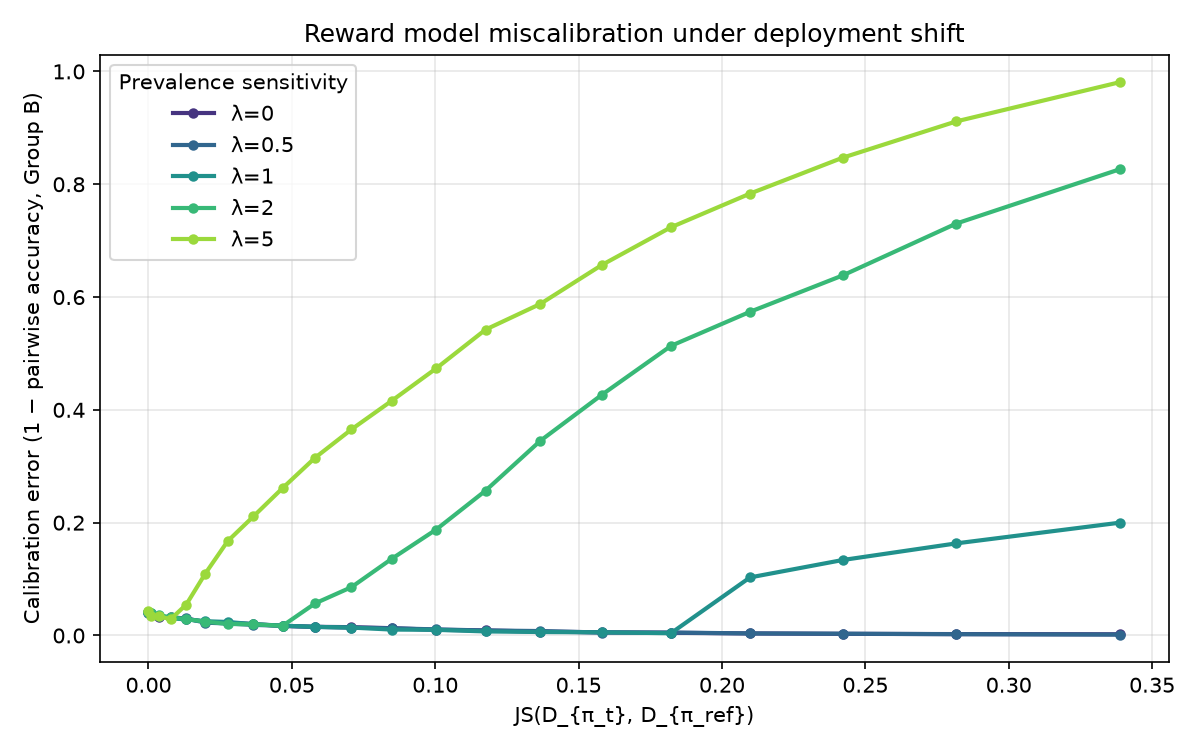
\includegraphics[width=\columnwidth]{figures/exp1_calibration_curve.png}
\caption{Experiment 1: calibration error and pairwise-accuracy collapse versus deployment shift, by prevalence-sensitivity $\lambda$. Global ranking is preserved while local pairwise accuracy collapses past a $\lambda$-dependent threshold.}
\label{fig:exp1}
\end{figure}

\subsection{Experiment 2: group-aware methods, including the oracle, fail}

We compare three conditions: (1) \emph{Standard RLHF}---a pooled Bradley--Terry reward model with KL-regularized policy optimization; (2) \emph{VPL (inferred)}---group-conditioned reward models with EM-inferred group membership \citep{poddar2024}; (3) \emph{VPL (oracle)}---group-conditioned reward models with oracle group labels. The oracle condition is the load-bearing design choice: it removes group-identification uncertainty entirely, so any remaining gap cannot be attributed to imperfect group inference. We report utility retention for Group B---realized \(U_B\) under the aligned policy divided by \(U_B\) under the performative optimum of Section~\ref{sec:gap}, computed by concave programming---as mean \(\pm\) standard deviation over 10 seeds, where each seed varies both the intrinsic-utility landscape and the preference sampling (Table~\ref{tab:retention}).

\begin{table}[t]
\centering
\small
\setlength{\tabcolsep}{3pt}
\begin{tabular}{@{}lccc@{}}
\toprule
$\lambda$ & Std.\ RLHF & VPL (inf.) & VPL (oracle) \\
\midrule
0.0 & 0.992 $\pm$ 0.014 & 0.977 $\pm$ 0.048 & 0.989 $\pm$ 0.014 \\
0.5 & 0.713 $\pm$ 0.131 & 0.623 $\pm$ 0.067 & 0.738 $\pm$ 0.137 \\
1.0 & 0.389 $\pm$ 0.363 & 0.152 $\pm$ 0.161 & 0.460 $\pm$ 0.323 \\
2.0 & $-$0.376 $\pm$ 0.776 & $-$0.904 $\pm$ 0.461 & $-$0.150 $\pm$ 0.667 \\
5.0 & $-$3.298 $\pm$ 2.267 & $-$4.221 $\pm$ 1.398 & $-$2.656 $\pm$ 2.029 \\
\bottomrule
\end{tabular}
\caption{Experiment 2: Group-B utility retention (mean \(\pm\) sd over 10 seeds). Retention \(1.0\) is the performative optimum; negative values mean the aligned policy is worse for Group B than the reference. Oracle group labels do not protect.}
\label{tab:retention}
\end{table}

\emph{Primary finding (reinforces the thesis).} All three methods collapse, and oracle group access provides no reliable protection. Mean retention falls from \(\approx 1.0\) at \(\lambda = 0\) to negative values by \(\lambda = 2\) for every method, including VPL-oracle (\(-0.15\) at \(\lambda = 2\), \(-2.66\) at \(\lambda = 5\)). Perfect group identity does not close the performative gap. This is the direct empirical form of the Section~\ref{sec:claim} claim, and it holds across seeds. The benchmark in every cell is the performative optimum, not the performatively stable policy (Section~\ref{sec:gap}). A worked instance of the two: at \(\lambda = 1\), \(v = (3, 2, 1, 0)\), the stable policy has \(\mu = 2\) and \(p = (1, 0, 0, 0)\) while the optimum has \(\nu = 1.5\) and \(p = (0.75, 0.25, 0, 0)\). In all 40 cells (10 seeds \(\times\) \(\lambda \in \{0.5, 1, 2, 5\}\)) the optimum's support strictly contains the stable policy's---support sizes 10--19 vs.\ 7--13 at \(\lambda = 0.5\), 12--21 vs.\ 10--19 at \(\lambda = 1\), 17--27 vs.\ 12--21 at \(\lambda = 2\), and 26--51 vs.\ 19--29 at \(\lambda = 5\)---so the diversity ordering of Section~\ref{sec:gap} holds in the published environments, not only in the closed form.

\emph{Secondary finding (resolved by multi-seed averaging).} No method ranking is statistically supported. The seed-to-seed standard deviations are large and the three methods' error bands overlap substantially at every \(\lambda > 0\). A single-seed run in which VPL-inferred appears to beat VPL-oracle does not survive averaging; across 10 seeds VPL-oracle's mean is at or above the others at every \(\lambda > 0\), but not separably so. The primary finding does not depend on any ordering: all methods, oracle included, exhibit a large gap that widens with \(\lambda\), with the \(\lambda = 0\) negative control holding at retention \(\approx 1.0\) (0.977--0.992) for every method.

\begin{figure}[t]
\centering
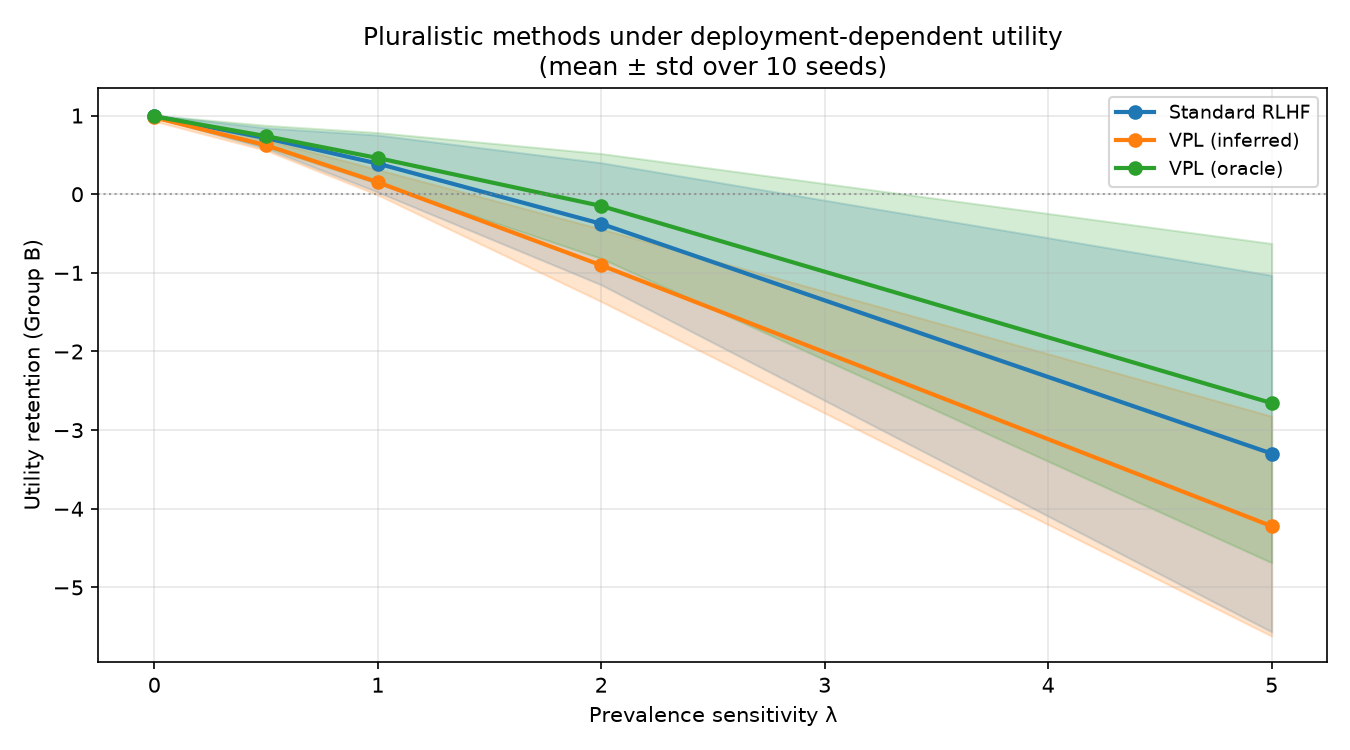
\includegraphics[width=\columnwidth]{figures/exp2_headline.png}
\caption{Experiment 2 (headline): utility retention versus $\lambda$ for all three methods. All start near 1.0 at $\lambda = 0$ and decline to negative retention as $\lambda$ grows, with the three curves interleaving rather than cleanly separating.}
\label{fig:exp2}
\end{figure}

\subsection{Metrics, construct-independence, and robustness}

Utility retention is the primary metric. Because it is defined against the assumed \(U_B\), on its own it is vulnerable to the circularity critique that the effect is baked into the utility definition. An earlier design proposed subgroup output divergence---the Jensen--Shannon (JS) divergence between Group A's and Group B's preferred distributions---as a construct-independent triangulation metric, predicting it would \emph{decline} with \(\lambda\) (flattening). In the executed runs it did the opposite in direction and was negligible in magnitude (pre-alignment \(\approx 0\); post-alignment rising only to \(\approx 0.0065\) JS at \(\lambda = 5\), against a ceiling near \(0.69\)), so we do not present it as corroboration. Instead we report a policy-level, construct-independent diversity/collapse metric that does not reference \(U_B\): the entropy (or effective support size) of the aligned deployed distribution and its JS divergence from \(\pi_{\text{ref}}\). This is the same construct \citet{kirk2024} use in documenting RLHF's reduction in output diversity relative to SFT, measured here on the deployed distribution rather than on model samples. We state plainly which claims rest on the construct-dependent metric (the size of the Group-B gap) and which rest on construct-independent observables (the concentration of the deployed distribution, and Experiment 1's pairwise-accuracy collapse, measured against sampled preferences rather than the assumed utility level).

The multi-seed result is the cleanest form of the thesis: method differences vanish into seed noise, so we report them as statistically indistinguishable and assert no ordering, while the shared collapse and the \(\lambda = 0\) control are robust. Retention going strongly negative at large \(\lambda\) reflects the linear penalty \(f = \mathrm{id}\), which directly opposes what alignment concentrates on; we therefore foreground the modest-\(\lambda\) regime where the qualitative gap is already clear, and rather than sweeping gentler synthetic forms we let Experiment 3 measure the actual form from a real judge (Section~\ref{sec:live}). The claim is the existence and \(\lambda\)-scaling of the gap, not its extreme magnitude.


\section{Experiment 3: verification and live-run details}
\label{app:synth}

\subsection{Protocol}
\label{app:exp3-protocol}

\textbf{Menu.} The frozen menu is \(100\) one-sentence descriptions of a city at night in ten designed style clusters of ten items: minimalist, ornate-poetic, slangy, formal, archaic, AI-house-style, technical, humorous, sensory-concrete, and aphoristic. Three examples, one per cluster: \emph{The city goes dark. Three windows hold out.} (minimalist); \emph{Beneath a diadem of trembling stars, the city exhales its silver breath into the velvet dark.} (ornate-poetic); \emph{A neon sign buzzes overhead, and the air smells like fried onions from a food cart.} (sensory-concrete). The three probe clusters are ornate-poetic, AI-house-style, and sensory-concrete (clusters 1, 5, and 8 in the tables). That the AI-house-style cluster---the menu's stand-in for the phrasing of Section~\ref{sec:intro}---is among the probes is by design, but nothing in the estimator treats it specially, and its measured \(\hat\lambda\) (\(+5.50\)) sits between the other two.

\textbf{Phase 1 design.} Prevalence is manipulated on the grid \(p \in \{0.02, 0.10, 0.25, 0.50, 0.80\}\) for the probe cluster, with the remaining mass spread uniformly over the other nine clusters. Each contextual-exposure cell elicits \(800\) pairs, each stated-prevalence cell \(300\), and each placebo and contamination cell \(150\) (the controls are lower-powered by design, which Appendix~\ref{app:redundancy} flags). Every pair is judged \(5\) times with the presentation order swapped, and the preference probability is the vote fraction; the contextual exposure block is \(20\) sentences sampled i.i.d.\ from the manipulated deployment distribution and resampled per pair and repeat. Intervals are percentile bootstraps with \(n_{\text{boot}} = 200\).

\textbf{Personas.} Both personas are fixed strings frozen before Phase 1; they ship verbatim in the released configuration alongside the response cache. Group A instructs the judge to select sentences ``for publication'' and to ``judge purely on the quality of the writing itself: vividness, precision, and craft.'' Group B instructs it to curate ``a daily feed'' whose ``readers follow the feed closely and see every sentence it publishes,'' and to ``pick sentences your readers will find rewarding to read today.'' Prevalence is never named in either persona; the exposure block is the only channel carrying it. The placebo swaps the prevalence summary for an irrelevant attribute (share of submissions from writers in one time zone), and the contamination arm pairs Group B's exposure block with Group A's persona and question.

\textbf{Phases 2--3.} In Experiment 3, \(\pi_{\text{ref}}\) is the softmax of the \emph{standardized} (zero-mean, unit-SD) \(\hat v\), not of raw \(\hat v\) as in Experiments 1--2: the judge's near-deterministic votes inflate the raw logit scale and its top item sits \(\approx 5\sigma\) out, so the raw softmax collapses onto that single item. Phase 2 fits \(\hat r\) on \(800\) reference-context pairs and evaluates \(400\) fresh pairs at each of \(t \in \{0, 0.2, \dots, 1.0\}\); the ``local'' region is the top-\(0.8\)-mass set of \(\pi_t\), and headline accuracies count only pairs on which the fresh judge is confident (\(|p_{\text{prefer}} - 0.5| \geq 0.3\)), since near-ties are a vote-noise floor. Phase 3 trains each method on \(800\) pairs per group from \(5\) simulated raters per group, optimizes with the same closed-form KL objective at \(\beta = 0.5\) and \(20\) EM iterations for VPL-inferred, and evaluates each resulting policy on \(400\) fresh pairs under the deployment that policy induces, over pair-sampling seeds \(\{0, 1, 2\}\). Two different solvers appear here and should not be confused. The surrogate-optimal comparator is the performative optimum of \(\hat U_B\) over the cluster-mix class, solved as a concave program (SLSQP; the same solver computes Experiment 2's optimum). The deployment-conditioned arm, by contrast, is a damped best-response iteration against the cluster-level surrogate (\(60\) steps, damping \(0.5\)) whose last iterate is used; its convergence was not verified, and no residual was logged.

\subsection{Gates and recovery}

\textbf{Phase 0 gates (live judge).} The initial menu's cluster-mean intrinsic-quality deviations ran from \(-1.21\) to \(+1.57\) item-SD under gpt-5.4. Six revisions brought the maximum cluster deviation to \(0.442\) item-SD, under the preset \(0.5\) gate, with the gate evaluated on a pooled fit over two independent 800-pair samples---single-sample cluster estimates carry \(\pm 0.15\)--\(0.2\) sampling noise, which is large against a \(0.5\) threshold (the final menu's own single-sample estimate read \(0.553\), above the gate), so the pooled fit is the recorded decision basis. The remaining live gates: cluster recoverability \(0.48\)--\(0.51\) against \(0.10\) chance, parse-failure rate \(0.000\), position bias \(0.46\)--\(0.54\), repeat agreement \(0.97\)--\(0.99\) no-context and \(0.73\)--\(0.77\) contextual (the contextual drop is expected---the exposure block is resampled per pair and repeat).

\textbf{Phase 0 gates (synthetic).} On the frozen menu the designed clusters are separable (cluster-label recoverability \(0.39\) against a chance rate of \(0.10\)) and intrinsic quality is balanced across clusters (maximum cluster-mean deviation \(0.43\) item-SD, within the preset bound), and the harness gates hold (parse-failure rate \(0.000\), position bias \(0.524\), near the \(0.5\) unbiased rate). The low synthetic repeat-agreement (\(\approx 0.58\)) is an artifact of near-tie pairs at the synthetic judge's temperature, not a harness fault.

Verification against a judge with a known \(\lambda\) is what converts ``did the experiment fail, or did the harness have a bug?'' into a testable question, so we report it in full here: the recovery below covers both families, all six probe cells, both null controls, and the functional-form machinery.

\textbf{Phase 1 recovery (synthetic).} For two synthetic families with true \(\lambda \in \{1.0, 2.0\}\) and three probe clusters each, the contextual-exposure estimate \(\hat\lambda\) is positive with a bootstrap CI excluding zero in all six cells (Table~\ref{tab:synth-recovery}). The two negative controls read \(\approx 0\) (placebo mean \(\hat\lambda = -0.11\), group-A contamination mean \(\hat\lambda = +0.34\), with \(0/6\) cells excluding zero in each). The magnitude ordering is preserved, though compressed (higher-sensitivity family mean \(\hat\lambda \approx 15.5\) vs.\ \(\approx 12.6\) across probe clusters; the families' per-cluster intervals overlap, so the ordering rests on point estimates). That true \(\lambda = 1.0\) yields \(\hat\lambda \approx 12.6\) is a consequence of Corollary~\ref{cor:did} rather than a caveat: only the composite \(g = \lambda f\) is identified, so \(\hat\lambda\) is a slope of \(\hat g\) on the elicited Bradley--Terry logit scale and absolute agreement with the generative \(\lambda\) was never predicted. Sign and ordering are the identified quantities, and both recover correctly. Per-cluster functional-form selection among linear, log, and threshold forms returns linear in five of the six contextual cells (threshold for cluster 8 at \(\lambda = 1.0\)), matching the generative \(f = \mathrm{id}\). Stated-prevalence \(\hat\lambda\) is also positive in all six cells but shows only weak rank agreement with contextual exposure (Spearman \(\rho = +0.50\) and \(-0.50\) for the \(\lambda = 1.0\) and \(\lambda = 2.0\) families---underpowered at \(n = 3\) clusters). The go/no-go gate (contextual \(\hat\lambda\) CI excludes 0 with consistent sign across \(\geq 2\) probe clusters in \(\geq 2\) families) returns GO.

\begin{table}[t]
\centering
\small
\begin{tabular}{@{}lccc@{}}
\toprule
Family & Cluster 1 & Cluster 5 & Cluster 8 \\
\midrule
\(\lambda = 1.0\) & \(+13.07\) & \(+11.49\) & \(+13.29\) \\
\(\lambda = 2.0\) & \(+15.48\) & \(+15.52\) & \(+15.50\) \\
\bottomrule
\end{tabular}
\caption{Synthetic-judge Phase 1 recovery: contextual-exposure \(\hat\lambda\) by probe cluster.}
\label{tab:synth-recovery}
\end{table}

\begin{figure}[t]
\centering
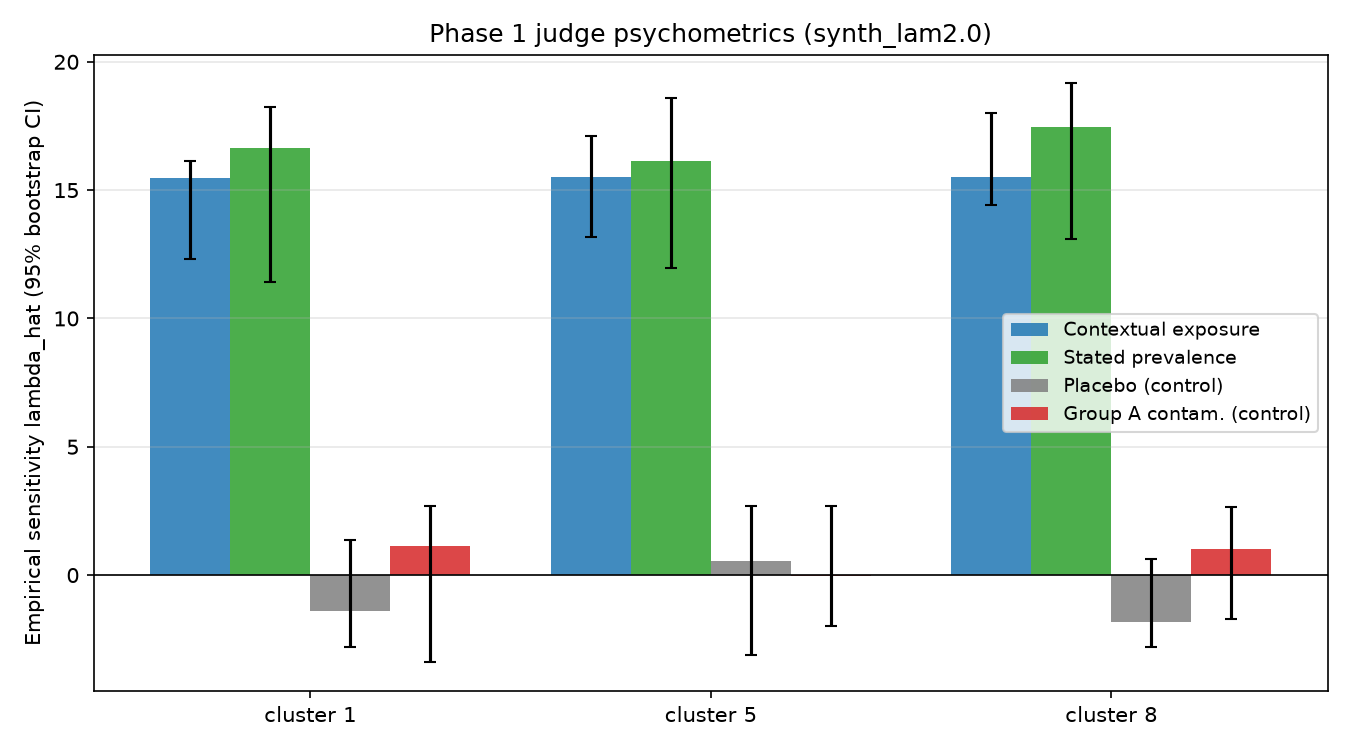
\includegraphics[width=\columnwidth]{figures/exp3_psychometrics.png}
\caption{Experiment 3 (synthetic-judge verification): recovered psychometrics \(\hat\lambda\) by probe cluster and prevalence-conditioning format. Contextual and stated formats recover a positive sensitivity with CIs excluding zero; placebo and group-A contamination controls sit at zero.}
\label{fig:exp3-synth-psyc}
\end{figure}

\begin{figure}[t]
\centering
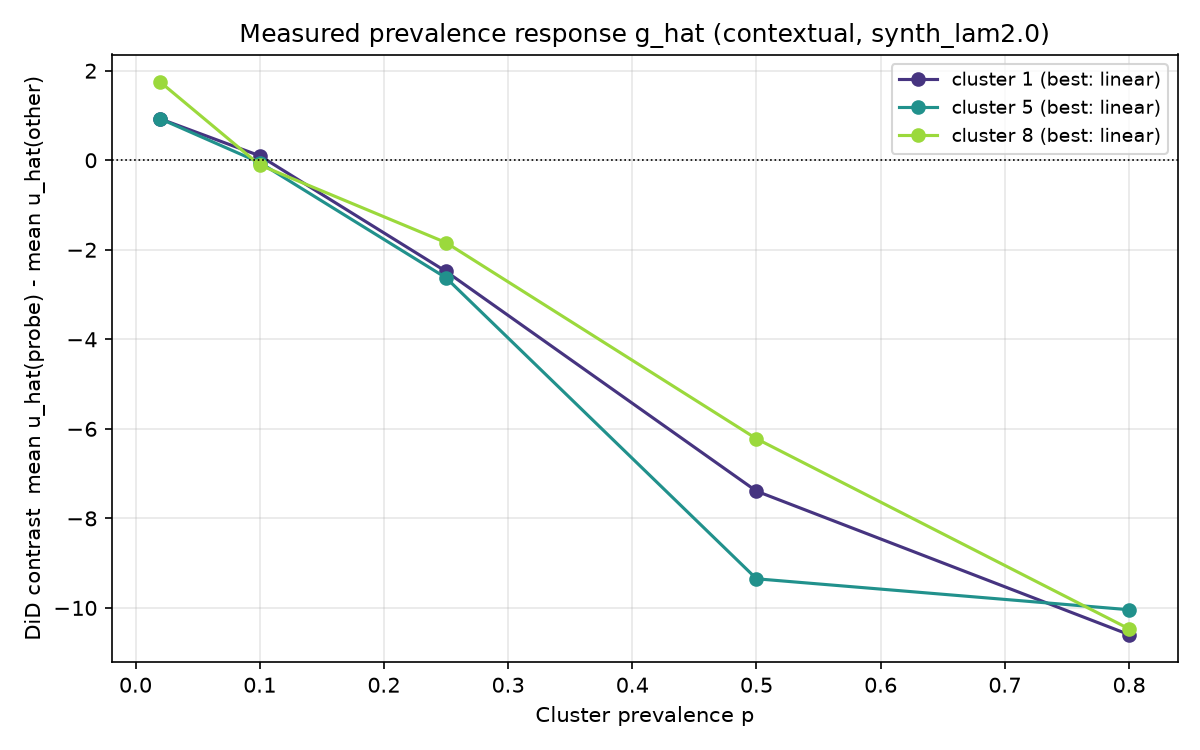
\includegraphics[width=\columnwidth]{figures/exp3_lambda_functional_form.png}
\caption{Experiment 3 (synthetic-judge verification, \(\lambda = 2.0\) family): measured prevalence-response \(\hat g\) (difference-in-differences contrast versus cluster prevalence \(p\)) for the contextual-exposure format, with the best-fit functional form per probe cluster. This is the empirical analogue of Section~\ref{sec:toy}'s assumed \(f\)-forms.}
\label{fig:exp3-fform}
\end{figure}

\textbf{Live psychometrics and Phases 2--3.} Figure~\ref{fig:exp3-live-psyc} visualizes the Phase 1 psychometrics of Table~\ref{tab:live-psychometrics}. Figure~\ref{fig:exp3-live-phase2} shows the live-judge miscalibration referenced in Section~\ref{sec:live}: Group B global accuracy and \(\rho\) decline while the Group A control stays flat, and within-region accuracy survives, isolating the degradation to cross-region comparisons. Figure~\ref{fig:exp3-live-phase3-gaps} shows the Phase 3 utility gaps of Table~\ref{tab:phase3-gaps}: oracle labels do not help, and the misspecified deployment-conditioned arm is worst.

\subsection{Phase 1 resampling unit and the in-context-redundancy alternative}
\label{app:redundancy}

\textbf{Resampling unit.} Every Phase 1 interval is a percentile bootstrap (\(n_{\text{boot}} = 200\)) over \emph{pairs}, resampled with replacement \emph{within} each prevalence level, with the Bradley--Terry fit and the difference-in-differences contrast recomputed on each resample. The item set and the probe-cluster membership are held fixed, so the intervals propagate pair-sampling and vote noise but not variability in which items---or which clusters---were drawn. This matters because prevalence is manipulated at the cluster level: with three probe clusters, the per-cell CIs cannot speak to between-cluster variability, and the cross-cluster consistency of Table~\ref{tab:live-psychometrics} (three of three significant, same sign, tight) is what carries that part of the evidence. A cluster-resampled interval would be the right object for a population-of-styles claim, and we do not make one.

\textbf{The redundancy alternative in full.} Any repeated material in a 20-item exposure block might depress judgments of text resembling it, with nothing to do with prevalence-sensitivity. Three features of the design bound that account. First, the estimand is a cluster-mean contrast---all ten items of the probe cluster against the other ninety---and the exposure block is sampled i.i.d.\ from \(D_\pi\) over the whole menu, so what elevated prevalence mostly shows the judge is \emph{other sentences sharing a style}, not the string under evaluation: at the top grid level (\(p = 0.8\), per-item mass \(0.08\)) an average block carries \(16\) probe-cluster items, of which only \(\approx 1.6\) are the evaluated item itself. Under i.i.d.\ 20-item blocks, moreover, roughly two-thirds of contextual judgments contain neither candidate verbatim (\(\approx 66\%\) at \(p = 0.02\), \(\approx 77\%\) at \(p = 0.8\), from the sampling design). The measured effect is therefore style-level, not literal-repetition-level. Second, the Group-A contamination arm sees exposure blocks built by the same sampler from the same deployment distributions over the same prevalence grid, differing only in the judge persona (and in the sampled pair set), and it stays null in two of three clusters---\(\hat\lambda = +0.12\) and \(+3.36\) in clusters 5 and 8 against Group B's \(+5.50\) and \(+5.47\). A persona-independent redundancy effect should appear equally in both arms; it does not. Phase 2 repeats the contrast at concentrated deployments: its Group A arm used the same contamination template (intrinsic persona plus matched exposure blocks from each \(\pi_t\)) and stayed near flat while Group B degraded (Section~\ref{sec:live}). Third, item-level verbatim repetition does produce a large effect on this judge---but it appeared separately and far more sharply in Phase 3 (the cluster-argmax policy realizing \(-3.9\); Section~\ref{sec:live}), which is evidence that the two are dissociable phenomena rather than one mechanism observed twice.

Where this defense is weakest: cluster 1's contamination cell at \(\hat\lambda = +4.61\) is close enough to that cluster's Group-B estimate (\(+5.82\)) that a style-level redundancy effect operating on both personas cannot be excluded there. The control cells are also lower-powered than the probe cells by design (\(150\) versus \(800\) pairs, so their intervals are more than twice as wide at equal noise), and their nulls are correspondingly weak evidence of absence: they rest on point estimates as much as on significance. The experiment that would settle it is an exposure format that is neither verbatim nor adjacent: exposure blocks drawn from a held-out set of same-style items, with the evaluated items themselves excluded from the block, which separates ``this style is everywhere'' from ``I have just read this sentence.''

\begin{figure}[t]
\centering
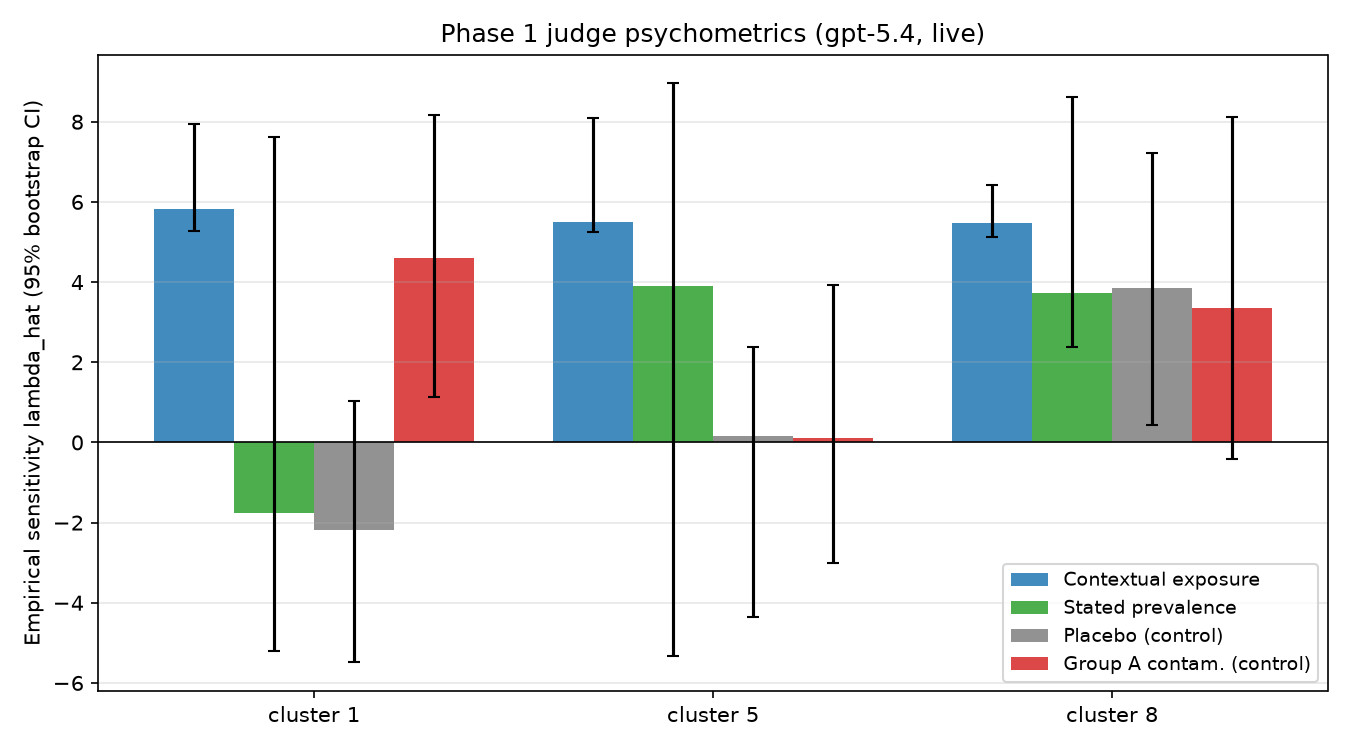
\includegraphics[width=\columnwidth]{figures/exp3_live_psychometrics.png}
\caption{Experiment 3 (live, gpt-5.4): recovered psychometrics \(\hat\lambda\) by probe cluster and prevalence-conditioning format, with placebo and contamination controls.}
\label{fig:exp3-live-psyc}
\end{figure}

\begin{figure*}[t]
\centering
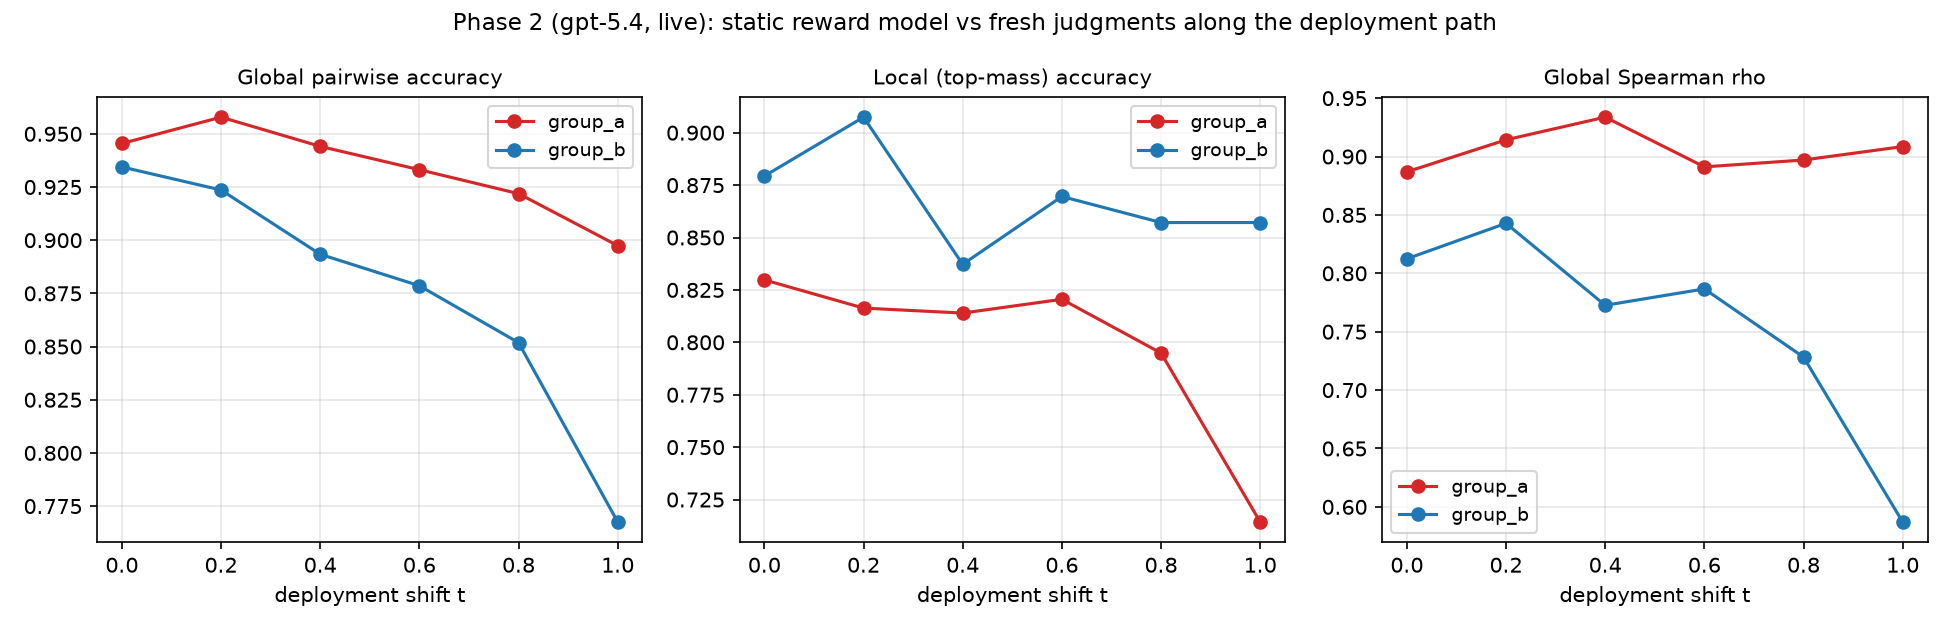
\includegraphics[width=\textwidth]{figures/exp3_live_phase2.png}
\caption{Experiment 3 (live, gpt-5.4): static-reward miscalibration under deployment shift---Group B global accuracy and \(\rho\) decline while the Group A control stays flat, and within-region accuracy survives (cross-region-not-within-region).}
\label{fig:exp3-live-phase2}
\end{figure*}

\begin{figure}[t]
\centering
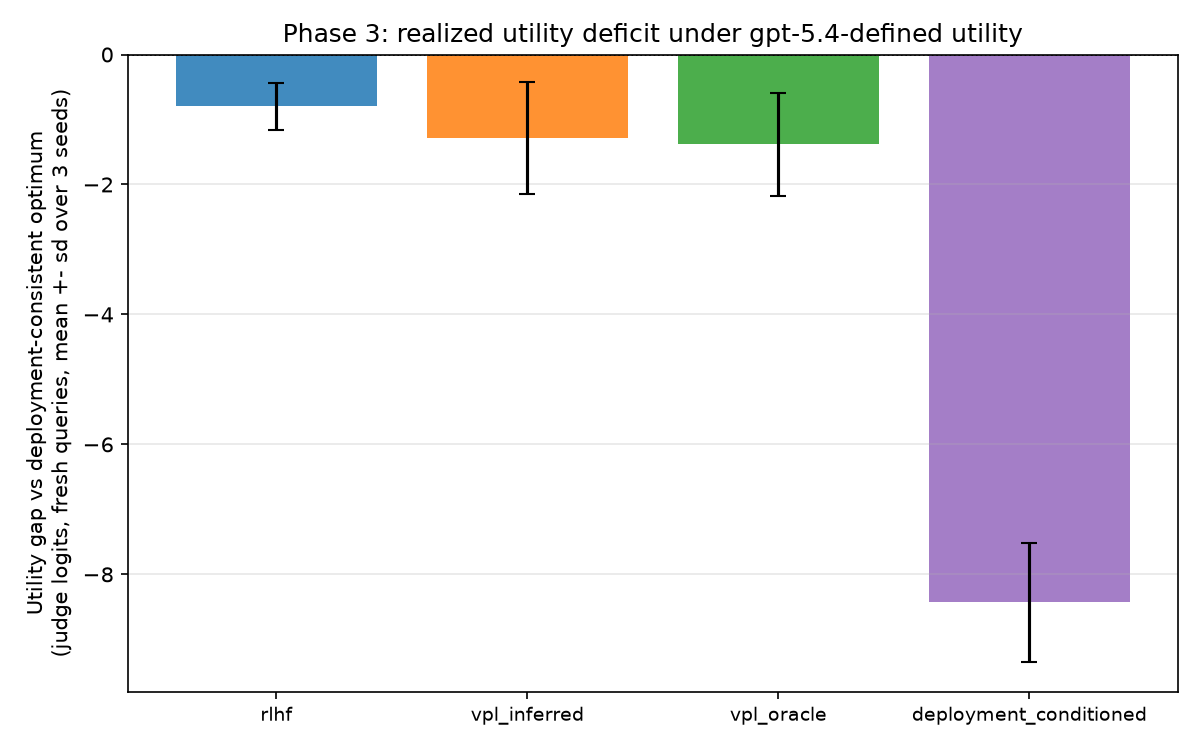
\includegraphics[width=\columnwidth]{figures/exp3_live_phase3_gaps.png}
\caption{Experiment 3 (live, gpt-5.4): utility gaps to the surrogate-optimal comparator under fresh-judge evaluation, with effective support per condition. Oracle labels do not help; the misspecified deployment-conditioned arm is worst.}
\label{fig:exp3-live-phase3-gaps}
\end{figure}


\section{Multilingual homogenization: the extended argument}
\label{app:multiling}

This appendix expands Section~\ref{sec:multiling}. It is an argument about mechanism, not a result: nothing here is demonstrated by our experiments, and we present it as a predicted signature that a future study could confirm or refute.

\textbf{What the empirical literature reports.} Two findings anchor the case. \citet{ryan2024} show that preference tuning narrows global representation: alignment shifts model outputs toward the norms of Western, English-speaking populations across languages, and reward models systematically prefer dominant-norm responses. \citet{naous2024} show that aligned models default to Western cultural entities and associations even when prompted in Arabic, under-producing the locally grounded alternatives a native speaker would expect. Both are typically read as consequences of training-data imbalance---dominant-norm text is over-represented in pretraining and in preference data, so the model learns it better.

\textbf{Why imbalance is an incomplete account.} The imbalance reading treats the target as fixed and the estimate as skewed: with balanced data and better group modeling, the argument goes, the reward model would recover each community's preferences. Deployment-dependence says something different. Community-grounded outputs derive part of their value from prevalence \emph{at the scale of the community that uses them}: an idiom, honorific, register choice, or culturally specific construction is valuable partly because it is the form that community actually uses, and its value changes when the deployed distribution changes what is common. This is the scale-indexed structure of Section~\ref{sec:dd-utility}: utility is defined against \(D_\pi^S\) for a community-level \(S\), while alignment optimizes against the globally aggregated \(D_\pi\). By the mechanism of Experiment 1, the reward model then becomes locally invalidated exactly where the global deployment concentrates---which for a minority-language community is precisely the region its own utility is defined over. On this account the failure is not an estimation error that more data fixes; it is a misspecification that survives arbitrarily good group modeling, which is what Experiment 2's oracle result demonstrates in the synthetic setting and Proposition~\ref{prop:nonident} explains.

\textbf{The multi-scale connection to the live judge.} Section~\ref{sec:live}'s Phase 3 found the live judge penalizing prevalence at two granularities at once---cluster-level style and item-level verbatim repetition---with the item-level effect far sharper. That is the same nested-scale structure in miniature, inside a single language: a policy can be deployment-consistent at one scale while being badly inconsistent at another, and which scale the alignment procedure models determines which failure it produces. The multilingual case is the version of this problem where the scales are communities rather than clusters, and Section~\ref{sec:open} poses the general form as open.

\textbf{What would test it.} The two accounts diverge on two measurable axes. First, dose-response: on the deployment-dependence account, homogenization should scale with the divergence between the deployed and reference distributions and show the threshold-gated shape of Experiment 1 rather than smooth degradation. Second, oracle robustness: it should persist when group identity is given rather than inferred, whereas the imbalance account predicts that group-conditioned modeling with balanced per-group data closes the gap. A study pairing per-community frequency-over-time corpus data with native-speaker ratings of high- versus low-prevalence forms would measure the prevalence-response \(g\) at community scale directly---the multilingual analogue of our Phase 1, and the measurement this paper does not have.

\end{document}
